\vspace{-0.5cm}
\section{Implementierung von Reglern \buchSeite{147}}
\vspace{-0.5cm}
Es wird eine \textit{minimale} Implementierung angestrebt, was bedeutet, dass die Anzahl
der Integratoren minimal sein soll. Wenn der gegebene Regler $G_R(s)$ vollständig
gekürzt ist, dann hat eine minimale Implementierung n Integratoren.
%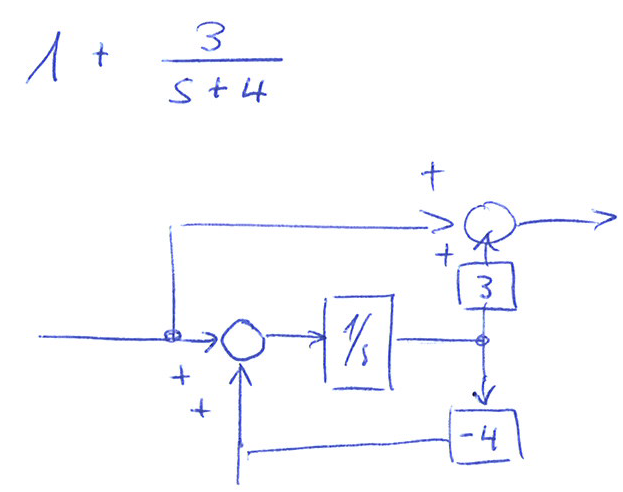
\includegraphics[width=5cm]{./images/implementierung2.png}
%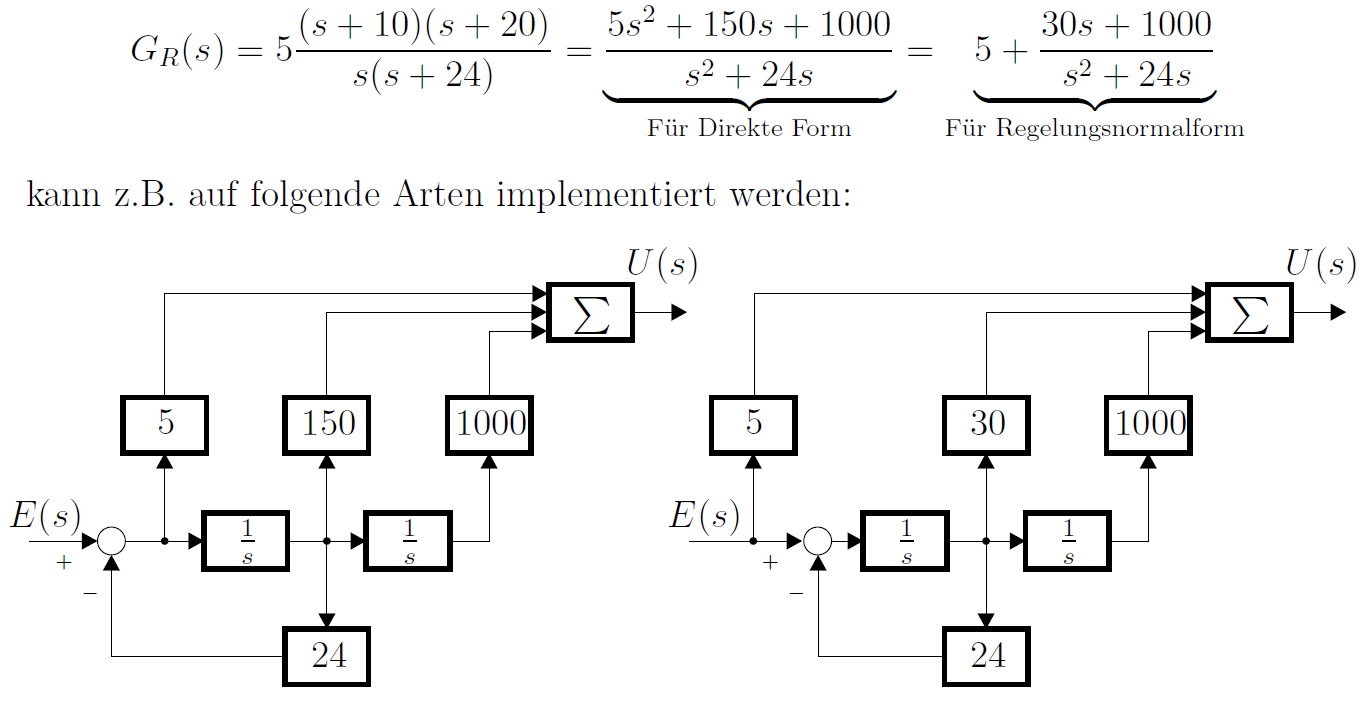
\includegraphics[width=10cm]{./images/implementierung.png}
\vspace{1cm}
\begin{center}
	\begin{tabu}{|p{0.25\textwidth}|p{0.7\textwidth}|}
	\hline
	\multicolumn{2}{|c|}{$G(s) = \frac{b_ms^m + b_{m-1}s^{m-1}+\dots + b_1s+b_0}{	s^n + a_{n-1}s^{n-1}+\dots + a_1s+a_0} \qquad (m\le n)$}\\[2mm]
	\hline
	\vspace*{-0.5cm}Direkte Form/ Direkte Form II
		& 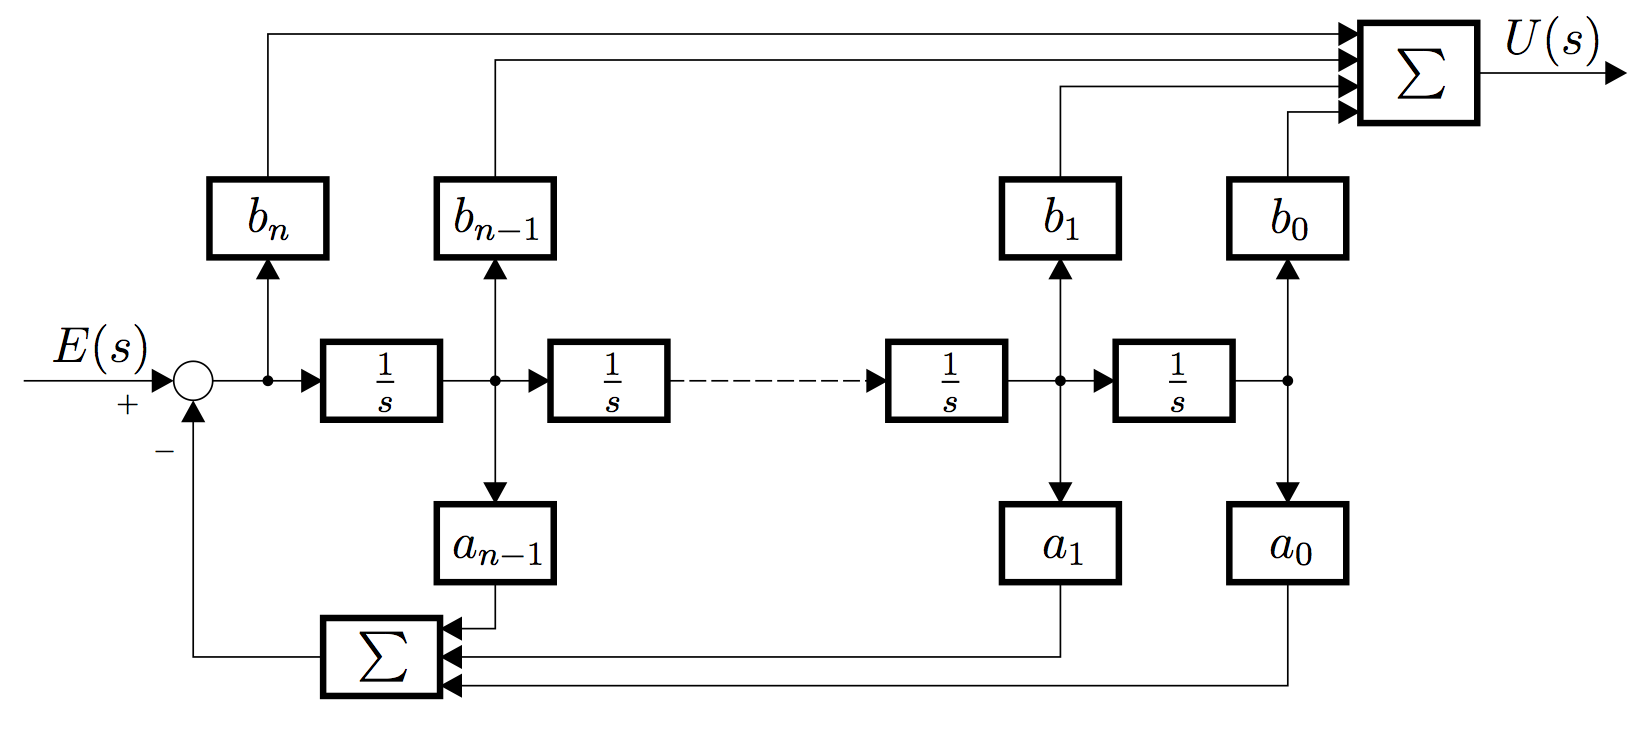
\includegraphics[width = \linewidth, height = 4cm, trim = 0 0 0 -5]{./images/DirekteForm2}\vspace*{-0.5cm}\\[2mm]
	\hline
	\vspace*{-0.5cm}Transponierte direkte Form/ Direkte Form I
		& 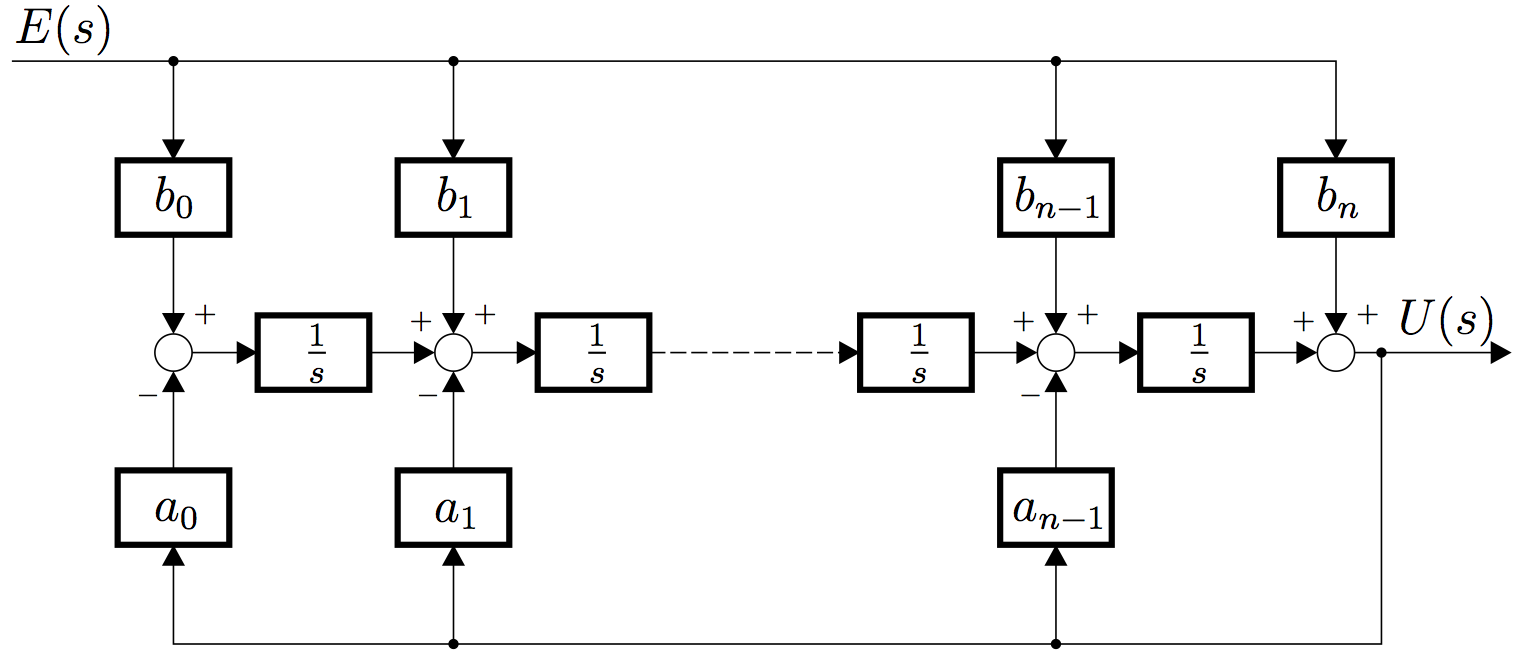
\includegraphics[width = \linewidth, height = 4cm, trim = 0 0 0 -5]{./images/DirekteForm1}\vspace*{-0.5cm}\\[2mm]
	\hline
	\multicolumn{2}{|c|}{$G(s) = d + \frac{b_ms^m + b_{m-1}s^{m-1}+\dots + b_1s+b_0}{s^n + a_{n-1}s^{n-1}+\dots + a_1s+a_0} \qquad (m < n)$}\\[2mm]
	\hline
	\vspace*{-0.5cm}Regelungsnormalform \buch{714}
		& 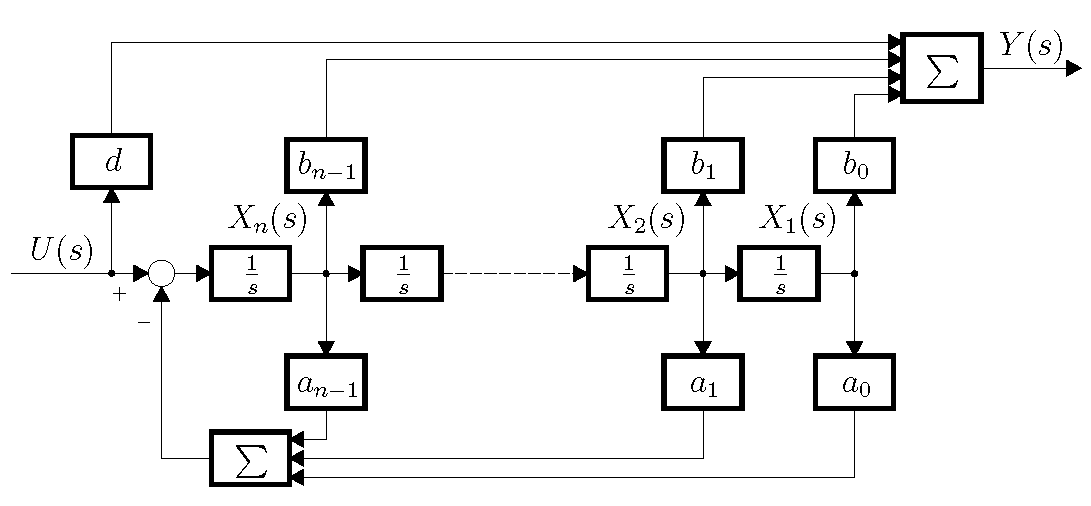
\includegraphics[width = \linewidth, height = 4cm, trim = 0 0 0 -5]{./images/regelungsnormalform}\vspace*{-0.5cm}\\[2mm]
	\hline
	\end{tabu}
\end{center}
\clearpage
